%%
%% $Id$
%%
%% Copyright (c) 2007-2008 Christian Fehler
%% Copyright (c) 2007-2008 Benjamin Mies
%%


\chapter{Wie erstelle ich einen Automaten?}

Wir wollen uns anhand des folgenden Beispiels anschauen, wie ein Automat
erstellt wird:\vspace{10pt}

\begin{figure}[h]
\begin{center}
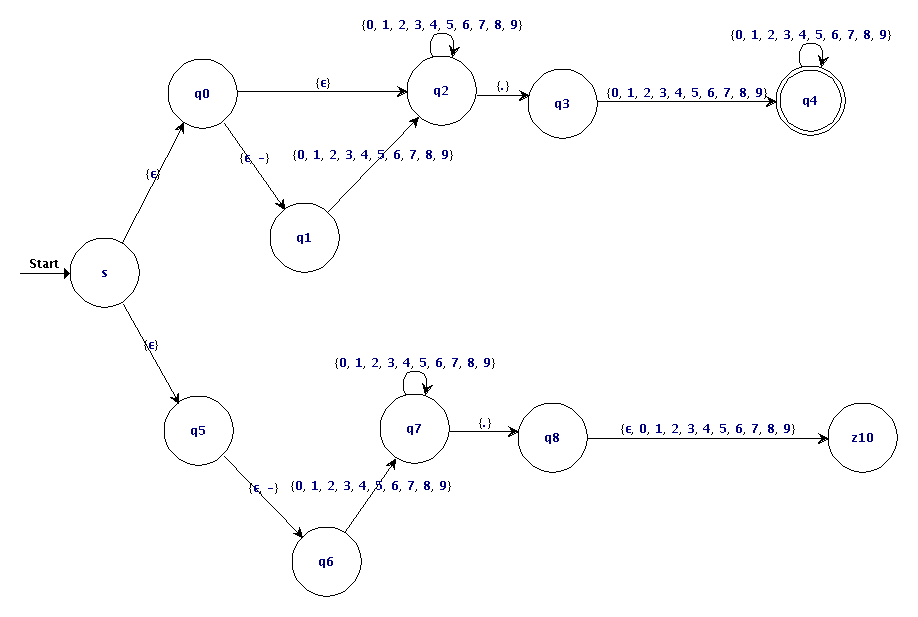
\includegraphics[width=12cm]{../images/enfa_example.png}
\end{center}
\end{figure}

\section{Neue Automat Datei anlegen}

Am Anfang müssen wir dazu erst einmal den "`Neu\ldots"' Dialog öffnen. Dort
wählen wir aus, dass wir einen Automaten erstellen wollen und klicken
auf "`Weiter"'.\vspace{10pt}

Im nächsten Dialog werden wir gefragt, von welchem Typ unser neuer
Automat sein soll. In unserem Beispiel handelt es sich um einen
"`$\epsilon$-NDEA"', welchen wir auswählen und mit "`Weiter"'
bestätigen.\vspace{10pt}

Dann müssen wir das gewünschte Alphabet für den neuen Automaten
angeben. Im Alphabet können alle Symbole werwendet werden, die nicht zur Syntax
der Eingabe gehören. Das bedeutet \Symbol{,}, \Symbol{\{}, \Symbol{\}} und
\SymbolEmpty{} können hier nicht verwendet werden. Symbole, welche länger als ein
Zeichen sind, müssen in Anführungszeichen angegeben werden.\vspace{10pt}

In dem Dialog sind an allen Stellen schon vordefinierte Werte eingetragen. Dabei
handelt es sich um die Vorgaben, die man als Standardwerte in den Einstellung
eingetragen hat. Wie man diese Standardwerte ändert, kann man in Kapitel
\ref{Preferences} nachlesen.\vspace{10pt}

Wir müssen noch die von uns benötigten Symbole angeben. Dazu tragen wir in das
Feld Alphabet "`\{\Symbol{0},\ \Symbol{1},\ \Symbol{2},\ \Symbol{3},\
\Symbol{4},\ \Symbol{5},\ \Symbol{6},\ \Symbol{7},\ \Symbol{8},\ \Symbol{9},\
\Symbol{-}\}"' ein. Damit haben wir alle benötigten Information eingegeben und
können den neuen Automaten durch Klick auf "`Fertig"' erstellen.\vspace{10pt}
\vspace{10pt} 

\begin{figure}[h]
\begin{center}
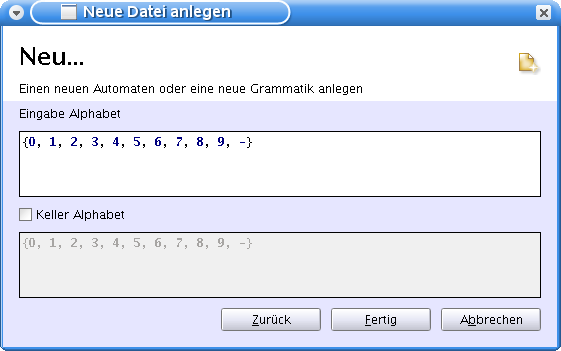
\includegraphics[width=8cm]{../images/new_dialog_machine.png}
\caption{Automat - Toolbar}
\end{center}
\end{figure}

Das für den Automaten angegebene Alphabet, lässt sich jeder Zeit über den Button
"`Dokument editieren"' nächträglich ändern.

\section{Zustände und Übergänge anlegen}

Um einen Automaten zu bearbeiten, müssen wir zuerst den entsprechenden Modus
auswählen. Folgende Modi sind in der Toolbar verfügbar:

\begin{figure}[h!]
  \begin{center}
    \begin{minipage}[t]{1cm}
      
\includegraphics[width=0.4cm]{../images/machineToolbar/mouse.png}
    \end{minipage}
    \begin{minipage}[t]{5cm}
      Maus Modus
    \end{minipage}
  \end{center}
\end{figure} 

\begin{figure}[h!]
  \begin{center}
    \begin{minipage}[t]{1cm}
      
\includegraphics[width=0.5cm]{../images/machineToolbar/state.png}
    \end{minipage}
    \begin{minipage}[t]{5cm}
      Neuer Zustand
    \end{minipage}
  \end{center}
\end{figure} 

\begin{figure}[h!]
  \begin{center}
    \begin{minipage}[t]{1cm}
      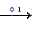
\includegraphics[width=0.5cm]{../images/machineToolbar/transition.png}
    \end{minipage}
    \begin{minipage}[t]{5cm}
      Neuer Übergang
    \end{minipage}
  \end{center}
\end{figure} 

\begin{figure}[h!]
  \begin{center}
    \begin{minipage}[t]{1cm}
      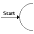
\includegraphics[width=0.5cm]{../images/machineToolbar/start.png}
    \end{minipage}
    \begin{minipage}[t]{5cm}
      Neuer Start Zustand
    \end{minipage}
  \end{center}
\end{figure}

\begin{figure}[h!]
  \begin{center}
    \begin{minipage}[t]{1cm}
      
\includegraphics[width=0.5cm]{../images/machineToolbar/final.png}
    \end{minipage}
    \begin{minipage}[t]{5cm}
      Neuer Akzeptierender Zustand
    \end{minipage}
  \end{center}
\end{figure} 


Da wir zu Beginn den Startzustand anlegen wollen, wählen wir "`Neuer Start
Zustand"' und klicken auf eine freie Fläche im unteren Teil, um den Zustand dort
zu erstellen. Um den Zustand nachträglich zu bearbeiten, müssen wir in den Maus
Modus wechseln. Den Konfigurationsdialog erreicht man dann über Doppelklick oder
das Kontextmenü. Über das Kontextmenü lässt sich ein Zustand auch wieder
löschen.\vspace{10pt}

Auf diese Weise lassen sich alle Zustände anlegen, die für den Beispielautomaten
benötigt werden. Nachdem wir alle Zustände angelegt haben, fehlen noch die
Übergänge zwischen den Zuständen. Daher wechseln wir in den "`Neuer Übergang"'
Modus. Um jetzt einen neuen Übergang anzulegen, klicken wir auf einen Zustand und
ziehen, bei gedrückter Maustaste, die Maus auf einen anderen Zustand. Beim
Loslassen öffnet sich der Konfigurationsdialog für Übergänge. In diesem Dialog
ziehen wir jetzt die Symbole, die in dem Übergang enthalten sein sollen, aus der
linken Liste mit allen Symbolen in die rechte Liste, welche die Übergangsmenge
repräsentiert. Als Hilfestellung wird im unteren Dia\-log der entstehende
Übergang angezeigt. Nach bestätigen durch "`OK"' wird der Übergang
angelegt.\vspace{10pt}

Die Übergänge lassen sich auf die gleiche Weise bearbeiten und löschen, wie es
bei den Zuständen möglich ist. Es gibt allerdings eine Besonderheit: Wenn man die
Maus anstatt über einem Zustand, über einem leeren Bereich los lässt, entsteht
beim Anlegen des Übergangs zusätzlich ein neuer Zustand.\vspace{10pt}

Diesen Vorgang wiederholen wir jetzt für alle Übergänge, die
für den Beispielautomaten benötigt werden. Wenn wir damit fertig sind, können
wir den Automaten noch validieren, um zu sehen, ob uns beim Anlegen der Zustände
und Übergänge irgendwelche Fehler unterlaufen sind. Diese Funktion erreicht man
über das Kontextmenü oder über den Menüpunkt "`Ausführen"'.\vspace{10pt}

Sollten die Zustände nicht ganz so optimal platziert sein, kann man
versuchen, über die Auto-Layout Funktion ein besseres Ergebnis zu
erreichen. Diese ist über "`Ausführen"' und "`Auto Layout"' oder über
das Kontextmenü erreichbar.

\section{Was fange ich mit einem Automaten an?}

Für einen erstellten Automaten gibt es folgende
Ver\-wen\-dungs\-möglich\-keiten.


\subsection{Bearbeiten per Übergangstabelle}

Die Übergänge eines Automaten können über die Tabelle bearbeitet werden. Diese
ist im rechten Teil des Fensters zu finden. Es ist möglich, neue Übergänge
anzulegen. Bestehende Übergänge können gelöscht oder editiert werden.\vspace{10pt}

Betrachten wir ein einfaches Beispiel. Wir legen zwei Zustände \State{z0} und
\State{z1} an und arbeiten auf dem Alphabet \{\Symbol{0}, \Symbol{1}\}. Die
Übergangstabelle besteht somit aus vier Spalten, in der ersten Spalte werden die
Zustände dargestellt, in der zweiten die Übergänge mit \Symbol{$\epsilon$} und in
den anderen die Symbole des Alphabets, also in unserem Fall je eine Spalte für
\Symbol{0} und \Symbol{1}.\vspace{10pt}

Um von \State{z0} nach \State{z1} einen $\epsilon$-Übergang anzulegen, muss die
erste Zeile mit \State{z0} bearbeitet werden. Da ein $\epsilon$-Übergang angelegt
werden soll, muss die zweite Spalte bearbeitet werden. Um dies umzusetzen, muss
auf die entsprechende Zelle doppelt geklickt werden. Es steht ein Parser zur
Verfügung, in den mit Komma getrennte Zustände eingetragen werden können. Die
Zustände müssen vorhanden sein. In userem Beispiel tragen wir also in der zweiten
Spalte, in der ersten Zeile den Zustand \State{z1} ein und bestätigen die Eingabe
mit Enter. Es wird, wie erwartet, ein $\epsilon$-Übergang von \State{z0} nach
\State{z1} angelegt.\vspace{10pt}

\begin{figure}[h]
\begin{center}
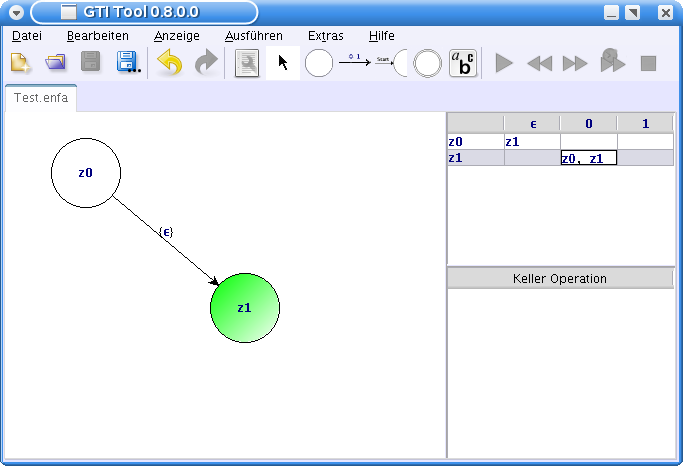
\includegraphics[width=12cm]{../images/machine_table.png}
\caption{Automat - Übergangstabelle bearbeiten}
\end{center}
\end{figure}

Als nächstes sollen zwei Übergänge auf einmal mit Symbol \Symbol{0} angelegt
werden. Beide sollen von Zustand \State{z1} ausgehen, der erste soll bei
\State{z0} enden, der zweite bei \State{z1}. Um dies umzusetzen, muss die Zeile
von \State{z1} und die Spalte von \Symbol{0} bearbeitet werden. Da der Übergang
zu den beiden Zuständen gehen soll, muss \State{z0}, \State{z1} eingetragen
werden.\vspace{10pt}

Das Löschen und Erweitern von Übergängen erfolgt analog.


\subsection{Vorlage für\ldots}
  
  Ein Automat kann als Vorlage für einen neuen Automaten benutzt werden. Dies
  sollte nicht mit "`Umwandeln in\ldots"' verwechselt werden. Es wird eine neue
  Datei angelegt, die alle Zustände und Übergänge des Ausgangsautomaten enthält.
  Allerdings kann man den Automatentypen neu festlegen.
  
\subsection{Wort-Navigation}
  
  Wir können für einen Automaten eine Wort-Navigation starten. Das bedeutet,
  dass wir ein Wort eingeben können, welches wir den Automaten verarbeiten lassen
  wollen und können dann schrittweise vor und zurück navigieren. Dabei werden
  die aktuell aktiven Zustände und Übergänge farblich hervorgehoben. Am Ende
  können wir dann sehen, ob der Automat das von uns gewählte Wort akzeptiert oder
  nicht. Dies wird über ein Statusfeld im unteren Fenster signalisiert. Es gibt
  auch die Möglichkeit, zu erkennen, ob ein Wort zu einem früheren Zeitpunkt der
  Navigation akzeptiert würde. Dies kann man anhand eines Rahmens um das aktuelle
  Wort Feld erkennen. Ein roter Rahmen steht dafür, dass das Wort bis zum
  aktuellen Symbol von unserem Automat nicht akzeptiert wird, ein grüner Rahmen
  hingegen gibt zu verstehen, dass es akzeptiert wird.\vspace{10pt}
  
  \newpage
  Während man sich im Wort-Navigations-Modus befindet, lässt sich der Automat
  nicht weiter bearbeiten. Das bedeutet, wir können Zustände und Übergänge weder
  anlegen noch löschen oder bearbeiten. Dies ist erst nach Verlassen dieses
  Modus wieder möglich.\vspace{10pt}
  
  \begin{figure}[h]
  \begin{center}
  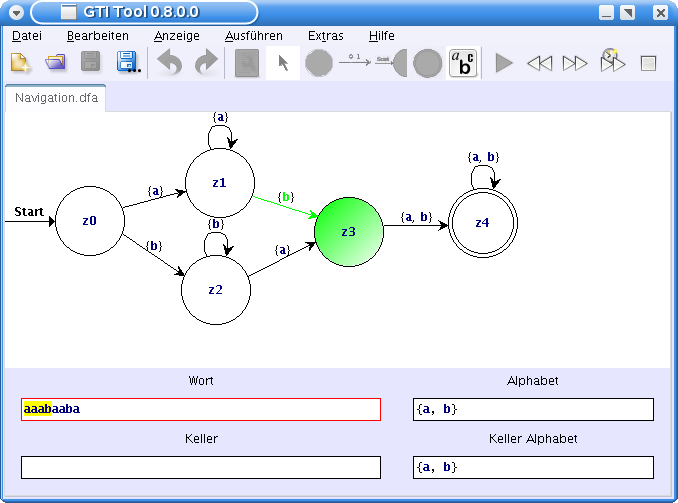
\includegraphics[width=12cm]{../images/dfa_navigation.png}
  \caption{Automat - Wort-Navigation}
  \end{center}
  \end{figure}
  
  Zur Wort-Navigation gelangt man über den Menüpunkt "`Ausführen"' und "`Wort
  eingeben"' oder direkt über den Button in der Toolbar. In dem Feld
  "`Wort"' können wir jetzt ein Wort eingeben. Als Hilfestellung sehen
  wir rechts neben dem Eingabefeld das aktuelle Alphabet mit den gültigen
  Symbolen.\vspace{10pt}
  
  Nachdem wir das Wort eingegeben haben, startet man die Navigation über
  "`Start"' in der Toolbar oder im Kontextmenü. Jetzt kann man mit "`Schritt vor"' und
  "`Schritt zurück"' durch das Wort navigieren. Es existiert auch noch ein
  automatischer Modus. Dabei wird nach einer kurzen Verzögerung das nächste
  Symbol gelesen. Dieser Modus lässt sich durch den Button "`Automatische
  Schritte"' aktivieren und deaktivieren.\vspace{10pt}

  \newpage
  Wenn man wissen möchte, über welche Pfade man zu den momentan aktiven Zuständen
  gelangt ist, kann man sich dies über "`Extras"' und "`Zustands Pfad"' anzeigen
  lassen. Es öffnet sich ein neuer Dialog mit einer Tabelle, in welcher für
  jeden aktiven Zustand der aktuelle Pfad angezeigt wird. Dabei wird als erstes der
  kürzeste Pfad angezeigt, und dann alle weiteren.\vspace{10pt}
  
    \begin{figure}[h]
  \begin{center}
  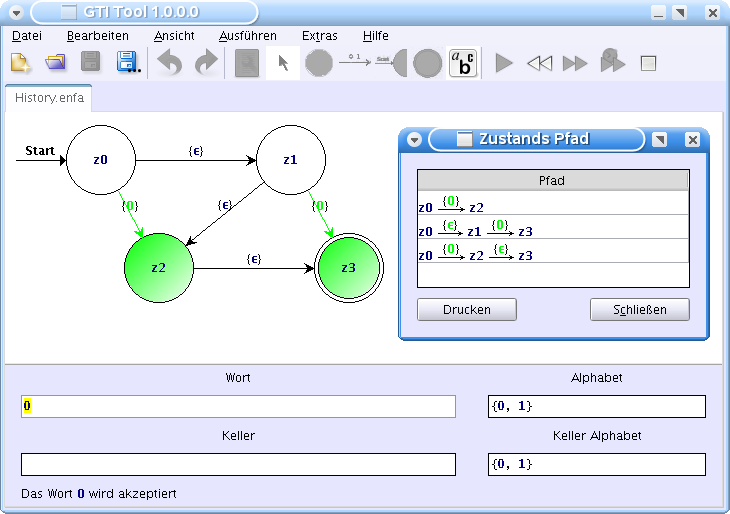
\includegraphics[width=12cm]{../images/history_path.png}
  \caption{Automat - Minimieren}
  \end{center}
  \end{figure}
  
  Um die Wort-Navigation zu beenden, klickt man einfach wieder auf den Button
  "`Wort eingeben"' in der Toolbar oder man wählt im Menü "`Ausführen"' den
  Punkt "`Automat bearbeiten"'. Jetzt befinden wir uns wieder im normalen Modus
  und wir können den Automaten wieder normal bearbeiten.
   
\subsection{Minimieren}
  
  Es besteht auch die Möglichkeit sich aus einem DFA den minimalen Automaten
  berechnen zu lassen. Für diese Funktion darf der Automat allerdings keine
  Fehler mehr enthalten, was wir durch eine Validierung ausschließen können. Das
  Minimieren startet man über den Menüpunkt "`Ausführen"' und
  "`Minimieren"'.\vspace{10pt}
  
  Es öffnet sich ein neuer Dialog mit einer Ansicht des Automaten und einer
  Tabelle. Der Automat sieht im Moment noch genau wie unser Ausgangsautomat
  aus. Wenn man allerdings jetzt auf "`Schritt vor"' klickt, werden als erster
  Schritt alle nicht erreichbaren Zustände entfernt. In der Outline wird
  angegeben, um welche Zustände es sich dabei handelt. Der zweite Schritt
  besteht darin, die erste Einteilung der Äquivalenzklassen vorzunehmen. Dazu
  unterteilen wir die Zustände des Automaten in akzeptierende und nicht
  akzeptierende Zustände. In der Automatenansicht werden immer die Zustände in
  der selben Farbe dargestellt, welche sich in einer Äquivalenzklasse befinden.
  Jetzt haben alle nicht akzeptierenden Zustände die gleiche Farbe. Gleiches 
  gilt für alle akzeptierenden Zustände, welche natürlich in einer anderen
  Farbe dargestellt werden.\vspace{10pt}
  
  \begin{figure}[h!]
  \begin{center}
  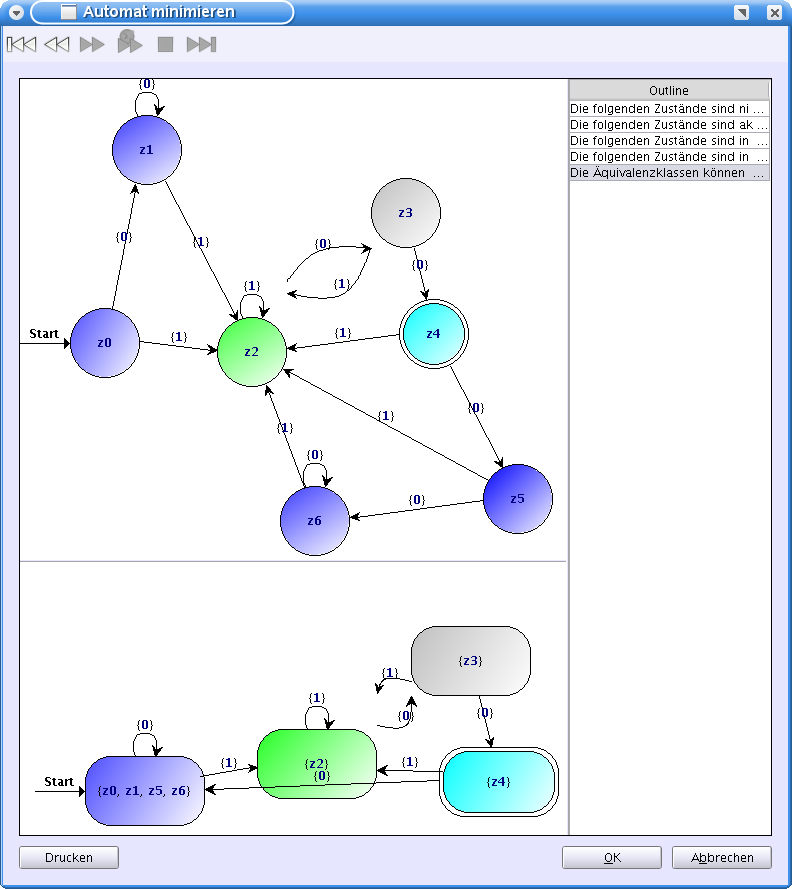
\includegraphics[width=12cm]{../images/minimize.png}
  \caption{Automat - Minimieren}
  \end{center}
  \end{figure}
  
  \newpage
  Man kann jetzt durch Klicken auf "`Schritt vor"' die Äquivalenzklassen weiter
  verfeinern. In der Outline wird angegeben, welche Zustände in eine eigene
  Äquivalenzklasse gekommen sind, und diese werden jetzt auch in einer anderen
  Farbe dargestellt. Gleichzeitig werden auch die Übergänge hervorgehoben, welche
  bei diesem Verfeinerungsschritt eine Rolle gespielt haben. Dabei beziehen sich
  die hervorgehobenen Übergänge immer auf den aktuell ausgewählten
  Tabelleneintrag.\vspace{10pt}
  
  Auf diese Weise kann man den Automaten jetzt Schritt für Schritt weiter
  verfeinern, bis keine Verfeinerung der Äquivalenzklassen mehr möglich ist. Wenn
  das der Fall ist, wird auch eine zweite Automatenansicht eingeblendet, dem
  entstandenen minimierten Automaten. Durch bestätigen mit "`OK"' wird jetzt
  eine neue Datei mit dem minimierten Automaten erstellt, mit welchem man dann
  weiter arbeiten kann.\vspace{10pt}
  
  Natürlich kann der Minimierungsprozess jederzeit abgebrochen werden. In diesem
  Fall wird keine neue Datei angelegt, man kann den Ausgangsautomaten weiter
  bearbeiten. \vspace{10pt}
  
  Wenn man in den Navigationsbereich des Dialogs schaut, stellt man fest, dass
  noch weitere Button verfügbar sind, auf welche jetzt noch nicht eingegangen
  wurde. Zunächst einmal gibt es die Button "`Bis zum Ende vor"' und "`An den
  Anfang zurück"'. Mit "`Bis zum Ende vor"' kann man alle Zwischenschritte
  überspringen, und gelangt direkt zur Ansicht des minimalen Automaten. "`An den
  Anfang zurück"' bewirkt genau das Gegenteil, und springt zur Ausgangsansicht
  zurück. Dann gibt es noch einen "`Schritt zurück"' Button, welcher einzelne
  Verfeinerungsschritte rückgängig macht. Und schlussendlich gibt es noch einen
  Button "`Automatische Schritte"', welcher nach einer kurzen Verzögerung
  automatisch den nächsten Schritt macht, bis der Minimierungsprozess
  abgeschlossen ist. Diese Funktion kann durch den "`Stop"' Button wieder
  deaktiviert werden.\vspace{10pt}
  
  Wenn man die neue Datei mit dem minimalen Automaten erstellen möchte, ohne sich
  die Minimierung im Detail anzuschauen, besteht jederzeit die Möglich\-keit,
  den Dialog mit "`OK"' zu bestätigen. Die Minimierung wird dann im Hintergrund
  beendet, man gelangt sofort zur Ansicht des neu entstandenen Automaten und
  kann mit diesem weiterarbeiten.
  
  
\subsection{Umwandeln in\ldots}\label{ConvertTo}
  
Es besteht auch die Möglichkeit, zwischen verschiedenen Automatentypen
umzuwandeln. Dabei stehen drei Umwandlungen zur Verfügung, die sich in den
verwendeten Schritten unterscheiden.

\begin{itemize}
  \item NDEA $\to$ DEA
  \item $\epsilon$-NDEA $\to$ DEA
  \item $\epsilon$-NDEA $\to$ NDEA
\end{itemize}

Betrachten wir als erstes einen einfachen NDEA mit zwei Zuständen \State{z0} und
\State{z1} und zwei Übergängen, der auf dem Alphabet \{\Symbol{a}, \Symbol{b}\}
arbeitet. Der Zustand \State{z0} ist ein Start-Zustand, der Zustand \State{z1}
ein akzeptierender Zustand. Der erste Übergang besteht zwischen \State{z0} und
\State{z1} mit Symbol \Symbol{a}, der zweite geht von \State{z0} in sich selbst
über, ebenfalls mit \Symbol{a}. Der Automat erkennt somit Wörter von der Form
$a^n$ für $n \geq 1$. Über den Eintrag "`Umwandeln in\ldots"' im Menüeintrag
"`Ausführen"' kann ausgewählt werden, in welchen Automaten umgewandelt wird. Da
wir einen NDEA angelegt haben, ist hier nur der DEA verfügbar. Wird dieser
ausgewählt, steht die schon aus anderen Ansichten bekannte Oberfläche zur
Verfügung. Auch hier kann in einzelnen Schritten, sowie automatisch navigiert
werden. Wird der Dialog mit "`OK"' bestätigt, steht in der Hauptansicht der
umgewandelte Automat zur Verfügung. Mit "`Abbrechen"' wird der Dialog einfach nur
geschlossen.\vspace{10pt}

\begin{figure}[h!]
\begin{center}
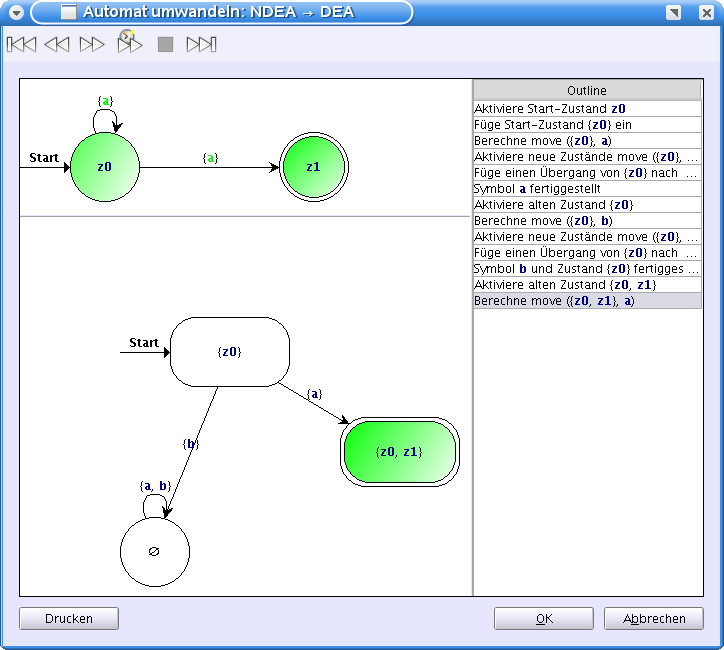
\includegraphics[width=12cm]{../images/convert_to.png}
\caption{Automat - Umwandeln in\ldots}
\end{center}
\end{figure}

\newpage
Werden die Schritte einzeln durchgegangen, ergibt sich folgender Ablauf:

\begin{enumerate}
  \item Der Start-Zustand \State{z0} wird aktiviert.
  \item In der unteren Ansicht wird der Start-Zustand \{\State{z0}\} angelegt.
  \item Die Übergänge mit dem ersten Symbol aus dem Alphabet, also \Symbol{a},
  werden hervorgehoben, um anzuzeigen, welche Zustände mit dem Symbol zu
  erreichen sind.
  \item In unserem Beispiel sind das die Zustände \State{z0} und \State{z1},
  die hervorgehoben werden.
  \item In der unteren Ansicht wird ein Übergang von \{\State{z0}\} nach
  \{\State{z0}, \State{z1}\} mit Symbol \Symbol{a} angelegt. Da dieser zweite
  Zustand in unserem Beispiel noch nicht existiert, wird er angelegt.
  \item Dieser Schritt zeigt an, dass das Symbol \Symbol{a} fertiggestellt ist.
  \item Da für den Zustand \{\State{z0}\} noch nicht alle Symbole betrachtet
  wurden, wird er aktiviert.
  \item Es wird die gleiche Berechnung wie bei Schritt drei durchgeführt,
  allerdings für Symbol \Symbol{b}. Da es in unserem Beispiel keinen Übergang
  von den betroffen Zuständen, bei uns nur \State{z0}, gibt, werden in der
  oberen Ansicht keine Übergänge hervorgehoben.
  \item Wie in Schritt vier werden die mit Symbol \State{b} erreichbaren
  Zustände in der oberen Ansicht hervorgehoben. In unserem Beispiel existiert
  kein Übergang von \State{z0} mit Symbol \Symbol{b}, deshalb werden in der
  oberen Ansicht keine Zustände hervorgehoben.
  \item Da wir in diesem Beispiel in einen DEA umwandeln, wird auch für diesen
  Fall ein Zustand angelegt und zwar der nicht akzeptierende Zustand
  \State{$\emptyset$}. Wird dieser Zustand während der Wort-Navigation
  erreicht, kann das Wort nicht mehr akzeptiert werden. Aus diesem Grund wird
  direkt der Übergang von diesem Zustand in sich selbst mit allen Symbolen des
  Alphabets angelegt. Es wird ein Übergang mit Symbol \Symbol{b} zu diesem
  Zustand \State{$\emptyset$} angelegt.
  \item Wie in Schritt sechs wird angezeigt, dass das Symbol \Symbol{b} fertig
  verarbeitet wurde. Da dieses Symbol das letzte im Alphabet ist, ist der
  Zustand \{\State{z0}\} fertiggestellt.
  \item In diesem Schritt wird der nächste, bis jetzt noch nicht verarbeitete,
  Zustand \{\State{z0}, \State{z1}\} in der unteren Ansicht hervorgehoben.
  Gleichzeitig werden in der oberen Ansicht die entsprechenden Zustände
  \State{z0} und \State{z1} hervorgehoben.
  \item Es folgt wieder das Hervorheben der Übergänge mit dem Symbol
  \Symbol{a}, wie dies in Schritt drei der Fall war.
  \item Wie in Schritt vier werden die Zustände \State{z0} und \State{z1}
  hervorgehoben.
  \item In Schritt fünf wurde der Übergang zum Zustand \{\State{z0},
  \State{z1}\} mit Symbol \Symbol{a} angelegt, gleiches geschieht jetzt in
  diesem Schritt. Da wir allerdings im Moment den gleichen Zustand bearbeiten,
  wird der Übergang von diesem Zustand in sich selbst angelegt.
  \item Das Symbol \Symbol{a} ist fertiggestellt.
  \item Da der Zustand \{\State{z0}, \State{z1}\} noch nicht fertiggestellt
  ist, wird er in beiden Ansichten wie gehabt hervorgehoben.
  \item Alle Übergänge, die von den Zuständen \State{z0} und \State{z1} mit
  Symbol \Symbol{b} ausgehen, werden hervorgehoben. In unserem Beispiel kommt
  das nicht vor.
  \item Die mit dem Symbol \Symbol{b} erreichbaren Zustände werden
  hervorgehoben, in unserem Beispiel ist das wieder kein Zustand.
  \item Deshalb wird in diesem Schritt wieder ein Übergang mit Symbol
  \Symbol{b} zu dem Zustand \State{$\emptyset$} angelegt.
  \item Der Zustand \{\State{z0}, \State{z1}\} ist mit dem letzten Symbol
  \Symbol{b} fertiggestellt. Da keine weiteren Zustände hinzugekommen sind, ist
  die Umwandlung fertiggestellt.
\end{enumerate}

Bei Betrachten des entstehenden DFA's erkennt man, dass dieser die gleichen
Wörter erkennt wie der ursprüngliche NFA. Der Dialog kann mit "`OK"' bestätigt
werden, womit ein neuer DFA angelegt wird. Es ist jetzt möglich, die Namen der
Zustände neu zu vergeben, wenn man mit dem Automaten weiterarbeiten möchte und
nicht die längeren Namen dargestellt haben möchte. Dazu kann man im Menü
"`Extras"' den Eintrag "`Zustandsnamen neu vergeben"' anklicken, wodurch die
Zustandsnamen neu, nach dem Muster \State{z0}, \State{z1} \ldots, vergeben
werden.\vspace{10pt}

Zu den anderen zwei Umwandlungarten gibt es noch kleinere Änderungen, die bei dem
durchgespielten Beispiel nicht betrachtet werden konnten. Wird ein
$\epsilon$-NDEA in einen NDEA umgewandelt, entfällt das Anlegen des Zustandes
\State{$\emptyset$}, es wird einfach kein Übergang mit dem entsprechenden Symbol
angelegt, da bei einem NFA nicht alle Symbole vorhanden sein
müssen.\vspace{10pt}

Wird ein $\epsilon$-NDEA umgewandelt, kommen jeweils zwei Schritte dazu. So wird
nach dem Aktivieren der alten Zustände, bei unserem Beispiel die Schritte eins,
sieben, etc., der $\epsilon$-Abschluss berechnet, es werden also auch alle
Zustände aktiviert, die mit $\epsilon$-Übergängen zu erreichen sind. Gleiches
gilt für das Anzeigen der neuen Zustände, bei unserem Beispiel in den Schritten
vier, neun etc., auch hier werden in einem einzelnen Schritt alle Zustände
hervorgehoben, die mit $\epsilon$-Übergängen zu erreichen sind.


\subsection{Umwandeln in\ldots (Potenzmenge)}
Der einzige Unterschied zwischen den Menüpunkten "`Umwandeln in\ldots"' und
"`Umwandeln in\ldots (Potenzmenge)"' ist, dass alle Zustände bei Verwendung der
Potenzmenge bereits zu Beginn angelegt werden, auch solche, die nicht benötigt
werden, die also nicht erreichbar sind. In dem in Abschnitt \ref{ConvertTo}
gewählten Beispiel wäre das der Zustand \{\State{z1}\}, da dieser nicht zu
erreichen ist und nur einen Übergang mit allen Symbolen zu dem Zustand
\State{$\emptyset$} hat. Wie solche Zustände im Anschluss entfernt werden können,
kann im Abschnitt \ref{ReachableStates} nachgelesen werden.


\subsection{Erreichbare Zustände}\label{ReachableStates}

Über den Menüeintrag "`Extras"' kann der Punkt "`Erreichbare Zustände"'
ausgewählt werden. In dem erscheinenden Dialog kann, wie in den anderen auch,
durch die einzelnen Schritte navigiert werden. Es geht hierbei darum, in
möglichst kleinen Schritten zu erkennen, welche Zustände erreichbar sind und
welche nicht. Der verwendete Algorithmus geht dabei in folgenden drei Schritten
vor:

\begin{itemize}
  \item Ein Zustand, der noch nicht berechnet wurde, wird ausgewählt (am Anfang
  wird mit dem Start Zustand begonnen)
  \item Die von dem ausgewählten Zustand aus zu erreichenden Zustände werden
  hervorgehoben, und falls sie noch nicht berechnet wurden, zu der Menge der
  noch zu berechnenden Zustände hinzugefügt
  \item Die bis jetzt erreichbaren Zustände werden hervorgehoben. Die Menge der
  noch nicht berechneten Zustände angezeigt 
\end{itemize}

\begin{figure}[h!]
\begin{center}
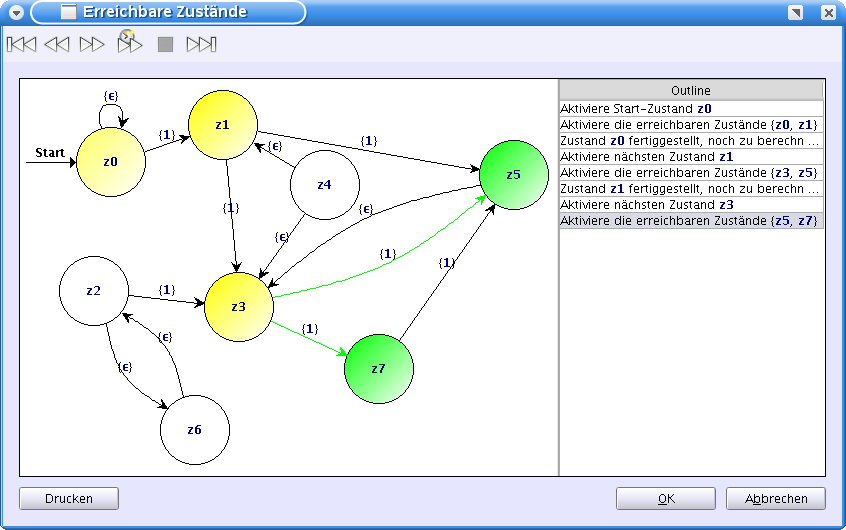
\includegraphics[width=12cm]{../images/reachable_states.png}
\caption{Automat - Erreichbare Zustände}
\end{center}
\end{figure}

Der Algorithmus läuft so lange, bis die Menge der noch nicht berechneten Zustände
leer ist. Am Ende werden alle erreichbaren Zustände farblich hervorgehoben. Wie
in den anderen Dialogen besteht jederzeit die Möglichkeit, den Dialog
abzubrechen, wobei er dann einfach geschlossen wird. Man hat auch jederzeit die
Möglichkeit, mit einem Klick auf "`OK"' die komplette Berechnung durchzuführen
und einen Automaten anzulegen, der nur noch die erreichbaren Zustände enthält.
